\chapter{KAJIAN PUSTAKA}

\section{Hasil Penelitian Terdahulu}
Penelitian ini tidak dibangun dari nol, melainkan merupakan pengembangan lanjut dari penelitian robotika yang telah berjalan. Penelitian ini secara spesifik mengisi celah (\textit{research gap}) yang tersisa dari dua penelitian pendahulu, terutama terkait integrasi sistem robot \textit{quadruped}, yaitu penelitian Darmawan pada aspek otonomi dasar dan penelitian Mahendra pada aspek perencanaan gerak berbasis bahasa alami.

\subsection{Pengembangan Robot \textit{Quadruped} untuk Estimasi Posisi Komponen \textit{Overheat} Pada Gardu Induk Berbasis Kamera Termal}

\begin{figure}[H]
    \centering
    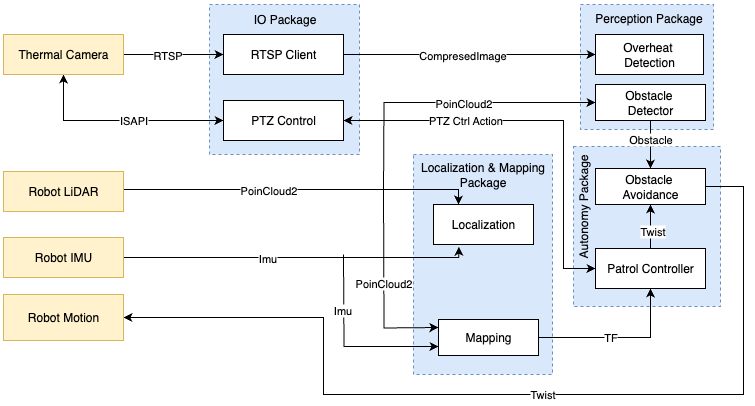
\includegraphics[width=0.8\textwidth]{Init/gambar/diagram_sistem_gusdar.png}
    \caption[Diagram Sistem robot Quadruped untuk Estimasi Posisi Komponen Overheat Pada Gardu Induk Berbasis Kamera Termal]{Diagram Sistem robot Quadruped untuk Estimasi Posisi Komponen Overheat Pada Gardu Induk Berbasis Kamera Termal \cite{Darmawan2025}}
    \label{fig:diagram_sistem_gusdar}																	
\end{figure}

Penelitian yang dilakukan oleh Darmawan \cite{Darmawan2025} mengembangkan sistem pemantauan otonom menggunakan robot \textit{quadruped} untuk mendeteksi kondisi \textit{overheat} pada komponen gardu induk. Arsitektur sistem dari penelitian tersebut, sebagaimana diilustrasikan pada Gambar \ref{fig:diagram_sistem_gusdar}, mengintegrasikan kamera termal dengan model deteksi objek YOLOv8s pada \textit{perception package} yang dioptimasi menggunakan OpenVINO untuk mengenali komponen kelistrikan, serta melakukan analisis suhu aktual secara langsung dari citra termal. Untuk pergerakannya pada \textit{autonomy package}, navigasi robot dikendalikan melalui kombinasi algoritma PID dan \textit{Pure Pursuit} agar dapat mengikuti lintasan patroli secara otonom, didukung oleh penghindaran rintangan menggunakan algoritma Braitenberg. Pada \textit{localization \& mapping package} Proses pemetaan lingkungan tiga dimensi dilakukan menggunakan algoritma SLAM FastLIO2 berdasarkan data LiDAR, dengan lokalisasi yang mengandalkan odometri. Seluruh operasi ini dipantau melalui sebuah \textit{control station} berbasis web yang menerima data telemetri dan aliran video secara waktu nyata melalui protokol WebSocket dan WebRTC. Hasil pengujian menunjukkan bahwa sistem ini berhasil mendeteksi \textit{overheat} dengan akurasi yang tinggi (mAP 0,8554) dan mampu beroperasi secara stabil dalam jarak transmisi hingga 100 meter, menjadikannya solusi inspeksi otonom yang andal.

Sistem ini terbukti andal dalam mendeteksi objek, tetapi mekanisme pengendalian dan navigasinya masih bersifat konvensional dan deterministik (\textit{hard-coded}). Robot hanya mampu bergerak ke lokasi yang koordinatnya telah di program secara eksplisit dalam kode sumber. Sistem ini tidak memiliki fleksibilitas untuk memahami instruksi yang bersifat semantik atau dinamis. Akibatnya, setiap perubahan skenario inspeksi memerlukan pemrograman ulang oleh ahli teknis, yang tidak efisien untuk penerapan lapangan yang dinamis. Selain itu, ketergantungan pada pemantauan telemetri manual masih membebankan beban kognitif yang tinggi pada operator.

\subsection{Interaksi Robot Manusia Berbasis \textit{Large Language Model} untuk Pembuatan \textit{Movement Plan} pada Robot \textit{Quadruped-legged}}

\begin{figure}[H]
    \centering
    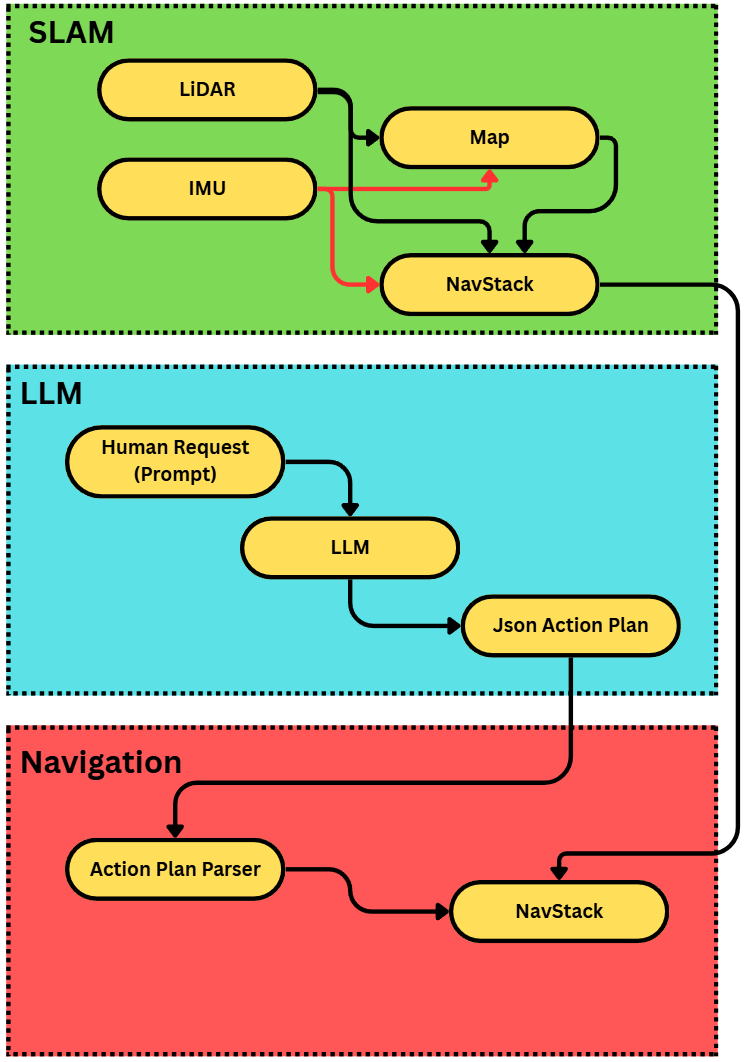
\includegraphics[width=0.5\textwidth]{Init/gambar/diagram_siste_vincent.png}
    \caption[Diagram Sistem Robot Quadruped untuk Interaksi Robot Manusia Berbasis Large Language Model untuk Pembuatan Movement Plan pada Robot Quadruped-legged]{Diagram Sistem Robot Quadruped untuk Interaksi Robot Manusia Berbasis Large Language Model untuk Pembuatan Movement Plan pada Robot Quadruped-legged \cite{Mahendra2024}}
    \label{fig:diagram_sistem_vincent}																	
\end{figure}

Di sisi lain, pendekatan berbeda dilakukan oleh Mahendra \cite{Mahendra2024} yang merancang sistem interaksi manusia-robot berbasis bahasa alami agar robot \textit{quadruped} dapat menyusun rencana pergerakan secara otonom. Arsitektur aliran data sistem tersebut, sebagaimana diilustrasikan pada Gambar \ref{fig:diagram_sistem_vincent}, mengelompokkan fungsionalitas ke dalam tiga modul utama, modul SLAM, modul pemrosesan bahasa (LLM), dan modul Navigasi. Penelitian ini menggunakan robot Jueying Lite 3 Pro yang dilengkapi sensor LiDAR Leishen C16, dengan pemetaan lingkungan menggunakan algoritma SLAM Fast-LIO. Peta yang dihasilkan kemudian dimodifikasi secara manual untuk menutupi batasan sensor, seperti menambahkan dinding virtual pada kaca transparan dan area tangga darurat. Sebagai pusat pemrosesan bahasa, sistem ini mengandalkan API Google Gemini yang diberikan instruksi khusus (\textit{prompt engineering}) mengenai lokasi target (\textit{waypoint}) dan batasan robot. LLM akan merespons perintah dari pengguna, baik berupa teks maupun suara melalui aplikasi web lokal berbasis Flask, dengan menghasilkan dokumen JSON yang berisi urutan perintah navigasi spesifik (seperti goto, halt, searchlab901, dan errmsg). Perintah errmsg didesain sebagai mekanisme keamanan agar LLM menolak permintaan yang tidak masuk akal atau membahayakan robot. Perintah JSON tersebut kemudian diterjemahkan oleh sebuah skrip \textit{parser} menjadi aksi navigasi yang dieksekusi oleh \textit{Navigation Stack} pada ROS. Evaluasi sistem menunjukkan bahwa LLM memiliki tingkat keberhasilan penyusunan rencana sebesar 85\% secara keseluruhan, bahkan mencapai 100\% pada instruksi kompleks maupun penanganan kegagalan. Kinerja navigasi robot juga sangat tinggi dengan rata-rata keberhasilan eksekusi mencapai 96,5\% dari 80 percobaan melintasi berbagai zona, di mana kegagalan kecil murni disebabkan oleh kendala perangkat keras fisik (seperti \textit{overheat} pada motor kaki). Hal ini membuktikan keandalan sistem dalam memproses instruksi percakapan sehari-hari menjadi logika navigasi JSON secara presisi.

Penelitian ini menawarkan fleksibilitas dalam input perintah dibandingkan metode konvensional, tetapi kelemahan mendasarnya terletak pada mekanisme eksekusi tugasnya yang bersifat menyeluruh. Sistem dirancang untuk menghasilkan seluruh rangkaian jalur navigasi di awal dan mengeksekusinya hingga selesai tanpa jeda. Desain alur kerja seperti ini membuat sistem tidak memiliki kemampuan untuk memvalidasi setiap tahapan pergerakan secara bertahap. Ketiadaan umpan balik di tengah misi ini menyebabkan hilangnya kemampuan operator untuk melakukan intervensi guna memodifikasi rencana di tengah jalan, padahal kontrol tersebut diperlukan untuk menyesuaikan strategi dengan kondisi lapangan yang berubah serta memastikan hasil setiap tahapan telah memenuhi standar yang diinginkan sebelum robot melanjutkan ke langkah berikutnya.

\section{Dasar Teori}

Bagian ini menguraikan berbagai landasan konsep, teknologi, dan kerangka teori yang menjadi pilar utama dalam pengembangan sistem pada penelitian ini. Keseluruhan teori ini digunakan untuk membangun pemahaman yang utuh mengenai bagaimana setiap komponen, baik dari sisi perangkat lunak maupun perangkat keras, saling terintegrasi dalam membangun arsitektur sistem inspeksi yang otonom dan adaptif.

\subsection{Lite3 \textit{Quadruped Robot}}

\begin{figure}[H]
    \centering
    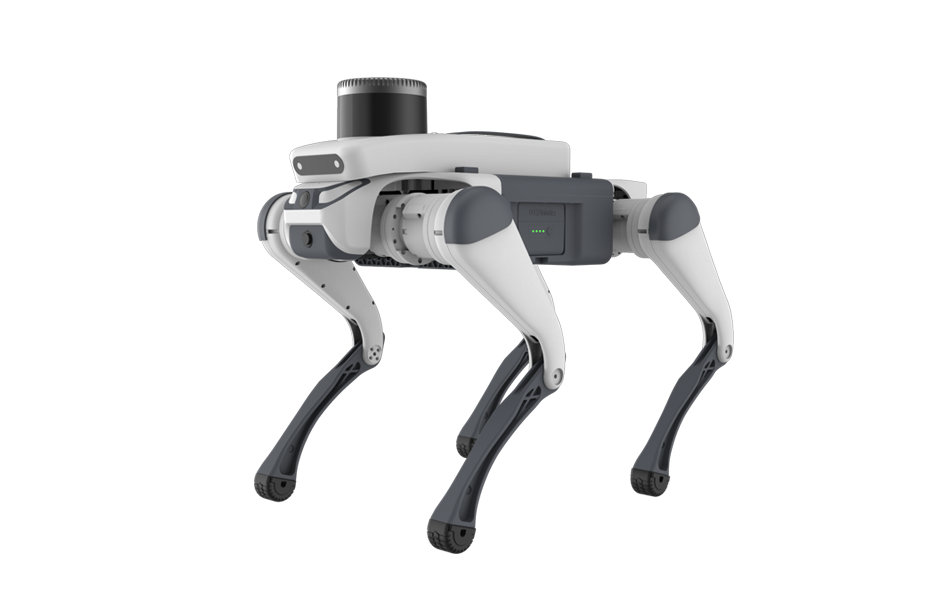
\includegraphics[width=0.5\textwidth]{Init/gambar/lite3.png}
    \caption[Robot Jueying Lite3]{Robot Jueying Lite3 \cite{maverick2026lite3}}
    \label{fig:lite3}
\end{figure}

Gambar \ref{fig:lite3} menunjukkan wujud fisik platform robot Jueying Lite3. Robot \textit{quadruped} merupakan kategori robot yang terinspirasi oleh mekanisme lokomosi hewan berkaki empat, mengintegrasikan desain mekanik, teori kontrol, dan kecerdasan buatan untuk beroperasi di lingkungan yang sulit dijangkau atau berbahaya bagi manusia \cite{li2025quadruped}. Konfigurasi berkaki empat menawarkan keseimbangan optimal antara mobilitas dan stabilitas, menjadikannya lebih stabil dibandingkan robot \textit{bipedal} (berkaki dua) sekaligus lebih lincah dan efisien secara energi dibandingkan robot \textit{hexapod} (berkaki enam) \cite{li2025quadruped}. Kemampuan adaptasi terhadap medan yang tidak rata, tangga, dan permukaan tidak terstruktur menjadikan robot \textit{quadruped} sangat cocok untuk aplikasi inspeksi infrastruktur, pemantauan lingkungan berbahaya, serta skenario pencarian dan penyelamatan di mana kendaraan beroda konvensional tidak dapat dioperasikan \cite{halder2023construction}.

Jueying Lite3 adalah platform robot \textit{quadruped} yang dikembangkan oleh DEEPRobotics dengan keperluan untuk riset dan aplikasi lapangan. DEEPRobotics merancang Lite3 dalam beberapa varian untuk memenuhi kebutuhan yang berbeda, yaitu Lite3 Basic yang merupakan robot anjing dengan kemampuan dasar, Lite3 Venture yang menambahkan konektivitas ethernet dan masukan daya eksternal, Lite3 Pro yang merupakan varian Venture dengan tambahan \textit{mini PC} di atasnya dan kamera kedalaman (\textit{depth camera}) untuk keperluan pengembangan, serta Lite3 Pro LiDAR yang merupakan varian Pro dengan tambahan sensor LiDAR. Salah satu keunggulan utama platform ini terletak pada keterbukaan arsitekturnya. Lite3 memiliki sistem perangkat lunak yang bersifat terbuka (\textit{open source}) sehingga pengembang dapat mengintegrasikan sensor tambahan, mengganti tumpukan perangkat lunak navigasi, atau menghubungkan sistem kecerdasan buatan eksternal tanpa perlu merombak desain dasar robot. Dalam penelitian ini, keterbukaan sistem tersebut dimanfaatkan untuk mengintegrasikan navigasi berbasis ROS dan agen LLM secara penuh ke dalam platform Lite3.

Secara arsitektur perangkat keras, khususnya pada varian Lite3 Pro LiDAR, robot ini dibangun di atas dua unit komputasi utama yang saling terhubung sebagaimana ditunjukkan pada Gambar \ref{fig:hardware_architecture}. Kedua unit tersebut adalah \textit{Motion Host} yang menangani kendali lokomosi dan \textit{Perception Host} yang mengelola pemrosesan data sensor. Keduanya dihubungkan melalui sebuah \textit{Router/Switch} internal untuk komunikasi data di dalam badan robot. 

\begin{figure}[H]
    \centering
    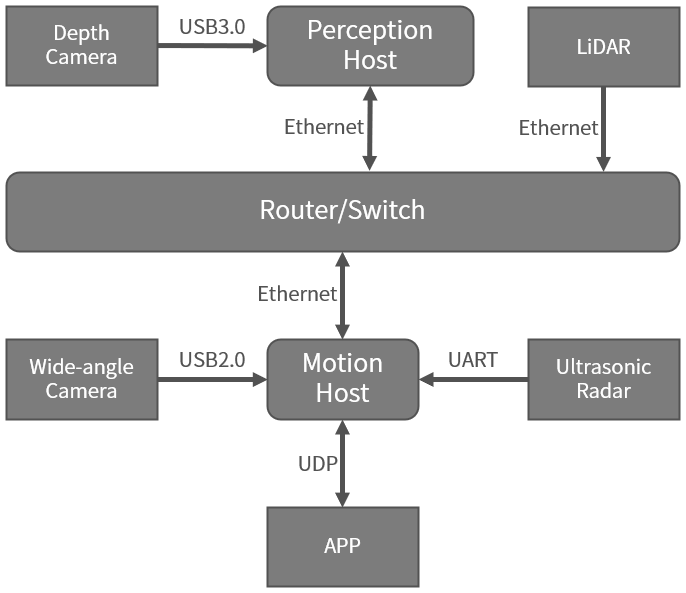
\includegraphics[width=0.5\textwidth]{Init/gambar/hardware_architecture.png}
    \caption[Arsitektur perangkat keras robot Lite3]{Arsitektur perangkat keras robot Lite3 \cite{deeprobotics2024motion}}
    \label{fig:hardware_architecture}
\end{figure}

\subsubsection{\textit{Motion Host}}
\textit{Motion Host} pada Lite3 bertanggung jawab atas seluruh aspek lokomosi fisik robot, meliputi koordinasi sendi, keseimbangan dinamis, dan perencanaan pola langkah (\textit{gait planning}). Sistem ini dikendalikan oleh prosesor berarsitektur ARM (RK3588) yang mampu menjalankan algoritma kontrol gerak berfrekuensi tinggi \cite{deeprobotics2024motion}. Setiap kaki robot terdiri dari tiga sendi aktif, yaitu HipX untuk gerakan abduksi-adduksi pinggul, HipY untuk fleksi-ekstensi pinggul, dan Knee untuk tekukan lutut. Masing-masing sendi digerakkan oleh motor DC berdaya tinggi yang dipasangkan dengan \textit{reducer} presisi dan \textit{absolute encoder} untuk memastikan ketepatan posisi sudut. Sistem ini juga dilengkapi mekanisme proteksi otomatis berupa penghentian gerakan saat suhu motor melebihi ambang batas (\textit{overtemperature protection}) dan deteksi kondisi jatuh (\textit{fall down protection}) yang secara langsung memutus perintah gerak demi keselamatan perangkat.

\subsubsection{\textit{Perception Host}}
\textit{Perception Host} pada Lite3 berfungsi sebagai indera utama yang menyediakan data spasial dan visual agar robot dapat memahami lingkungan di sekitarnya. Subsistem ini ditenagai oleh unit komputasi NVIDIA Jetson Xavier NX yang menyediakan akselerasi GPU untuk menjalankan algoritma persepsi secara \textit{real-time} \cite{deeprobotics2024perception}. Robot ini dilengkapi dengan dua jenis sensor utama yang bekerja secara komplementer. Sensor pertama adalah kamera kedalaman Intel RealSense D435i yang mampu menghasilkan peta kedalaman (\textit{depth map}) dan citra warna (RGB) secara simultan, menyediakan informasi jarak dan visual dari objek di sekitar robot. Sensor kedua adalah LiDAR 3D yang menghasilkan awan titik (\textit{point cloud}) tiga dimensi beresolusi tinggi untuk pemetaan dan lokalisasi spasial. Kedua sensor ini bekerja bersama untuk memberikan representasi lingkungan yang lengkap, di mana data LiDAR digunakan untuk membangun peta 3D dan menentukan posisi robot melalui algoritma SLAM.

\subsubsection{Komunikasi Antar \textit{Motion Host} dan \textit{Perception Host}}

\begin{figure}[H]
    \centering
    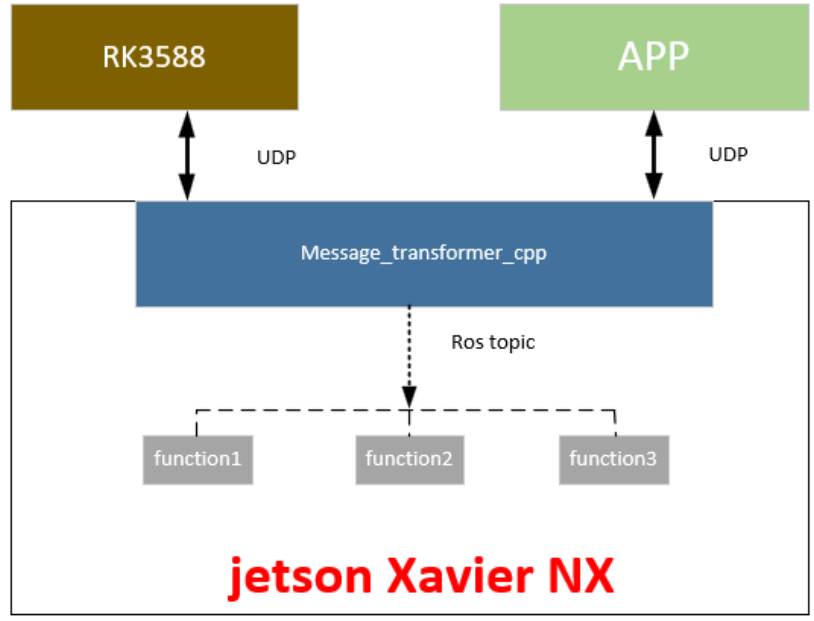
\includegraphics[width=0.6\textwidth]{Init/gambar/lite3_com_diagram.png}
    \caption[Diagram komunikasi antara \textit{Motion Host} dan \textit{Perception Host} pada robot Lite3]{Diagram komunikasi antara \textit{Motion Host} dan \textit{Perception Host} pada robot Lite3 \cite{deeprobotics2024motion}}
    \label{fig:lite3_com_diagram}
\end{figure}

Seperti yang diilustrasikan pada Gambar \ref{fig:lite3_com_diagram}, komunikasi antara \textit{Motion Host} dan \textit{Perception Host} dijalankan melalui protokol \textit{User Datagram Protocol} (UDP) yang bersifat ringan dan berlatensi rendah, sehingga sangat krusial untuk sistem kendali gerak yang membutuhkan respons waktu-nyata (\textit{real-time}). Komunikasi ini bersifat dua arah  dan melibatkan konversi format data di setiap sisinya, karena kedua unit komputasi menggunakan sistem operasi yang berbeda yaitu, \textit{Motion Host} (RK3588) beroperasi di atas sistem operasi \textit{real-time} QNX, sedangkan \textit{Perception Host} (Jetson Xavier NX) beroperasi di atas Linux dengan ekosistem ROS.

Pada arah dari \textit{Motion Host} ke \textit{Perception Host}, data status robot yang dihasilkan oleh sistem QNX pada RK3588 dikemas ke dalam paket UDP dengan format yang kompatibel dengan protokol QNX. Paket-paket ini kemudian diterima oleh modul perantara yang berjalan di Jetson Xavier NX, di mana data tersebut dikonversi dari format QNX menjadi pesan-pesan standar ROS dan diterbitkan ke \textit{topics} yang relevan. Dengan demikian, berbagai modul fungsional yang berjalan di atas ROS pada \textit{Perception Host} dapat mengonsumsi data dari \textit{Motion Host} melalui mekanisme \textit{subscribe} yang standar. Sebaliknya, pada arah dari \textit{Perception Host} ke \textit{Motion Host}, data perintah pergerakan yang dihasilkan oleh navigasi ROS dikemas ulang oleh modul perantara dari format pesan ROS menjadi format UDP yang dapat dipahami oleh sistem QNX pada \textit{Motion Host}. Paket perintah ini kemudian dikirimkan melalui UDP ke RK3588 untuk dieksekusi secara langsung oleh pengendali sendi dan algoritma kendali gerak. 

\subsection{\textit{Robot Operating System} (ROS)}

\textit{Robot Operating System} (ROS) adalah sebuah kerangka kerja (\textit{framework}) perangkat lunak yang fleksibel dan terdistribusi untuk pengembangan sistem robotik. Meskipun bernama sistem operasi, ROS bukanlah sistem operasi dalam artian tradisional seperti Windows atau Linux, melainkan sebuah \textit{middleware} yang berjalan di atasnya. ROS menyediakan layanan standar sistem operasi seperti abstraksi perangkat keras, kontrol perangkat tingkat rendah, implementasi fungsionalitas yang umum digunakan, penyampaian pesan antar proses, dan manajemen paket \cite{quigley2009ros}. Keunggulan utama ROS terletak pada ekosistemnya yang luas, memungkinkan integrasi berbagai driver sensor dan algoritma navigasi tanpa perlu membangun sistem dari nol. Dalam penelitian ini, seluruh infrastruktur perangkat lunak robot \textit{quadruped} dibangun di atas ekosistem ROS sebagai tulang punggung komunikasi dan koordinasi antar-modul, mulai dari persepsi sensor hingga eksekusi perintah navigasi.

\subsubsection{Arsitektur \textit{Node} dan \textit{Master}}
Arsitektur ROS dibangun berdasarkan komponen perangkat lunak independen yang disebut \textit{Nodes}. Setiap \textit{node} adalah sebuah proses komputasi yang bertanggung jawab atas tugas spesifik, seperti mengolah data kamera, merencanakan jalur, atau mengendalikan motor servo. Sifat modular ini memungkinkan tim pengembang untuk mengerjakan berbagai bagian dari sistem robot secara paralel dan independen. Agar \textit{node-node} ini dapat saling menemukan dan berkomunikasi, ROS menggunakan sebuah program inti yang disebut ROS Master (\textit{roscore}). Master menyediakan layanan registrasi nama dan pencarian (\textit{lookup}), yang memungkinkan \textit{node} pengirim dan penerima data untuk membuat koneksi \textit{peer-to-peer}. Arsitektur modular ini memungkinkan sistem robot inspeksi untuk menambahkan atau mengganti modul sensor dan navigasi tanpa harus merombak keseluruhan sistem.

\subsubsection{Mekanisme Komunikasi}

\begin{figure}[H]
    \centering
    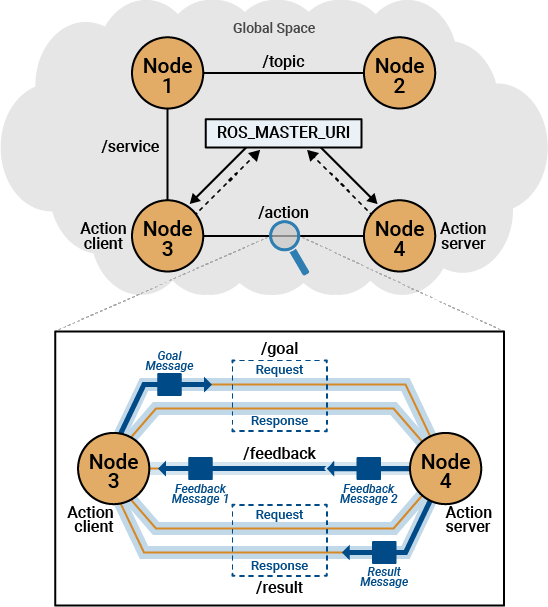
\includegraphics[width=0.6\textwidth]{Init/gambar/ros_actions.png}
    \caption[Diagram komunikasi antar-node dalam ROS]{Diagram komunikasi antar-node dalam ROS \cite{mathworks2025ros}}
    \label{fig:ros_communication}
\end{figure}

Mekanisme alur komunikasi antar-node dalam ROS sebagaimana diilustrasikan pada Gambar \ref{fig:ros_communication} difasilitasi oleh tiga mekanisme utama yang disesuaikan dengan kebutuhan pertukaran data yang berbeda:

\begin{enumerate}
    \item \textbf{Topics:} Mekanisme komunikasi asinkron yang menggunakan model \textit{publish-subscribe}. Sebuah \textit{node} (publisher) menyiarkan pesan ke sebuah \textit{topic} tertentu tanpa perlu mengetahui siapa penerimanya. \textit{Node} lain (subscriber) yang berlangganan ke topik tersebut akan menerima data secara \textit{real-time}. Mekanisme ini ideal untuk aliran data sensor berkelanjutan, seperti data LiDAR atau video stream.
    
    \item \textbf{Services:} Mekanisme komunikasi sinkron yang menggunakan model \textit{request-response}. Sebuah \textit{node} mengirimkan permintaan (\textit{request}) dan menunggu hingga \textit{node} penyedia layanan memprosesnya dan mengirimkan balasan (\textit{response}). Mekanisme ini cocok untuk tugas sesaat yang membutuhkan konfirmasi langsung, seperti menyalakan lampu LED atau mengubah mode operasi robot.
    
    \item \textbf{Actions:} Mekanisme komunikasi yang dirancang untuk tugas jangka panjang yang memerlukan waktu untuk diselesaikan dan membutuhkan umpan balik berkelanjutan. Berbeda dengan \textit{Services} yang memblokir proses hingga selesai, \textit{Actions} memungkinkan robot untuk membatalkan tugas di tengah jalan dan memberikan status progres secara berkala. Ini adalah mekanisme fundamental dalam navigasi robot, misalnya saat robot bergerak dari titik A ke titik B \cite{quigley2009ros}.
\end{enumerate}

\subsubsection{ROS \textit{Navigation Stack}}

\begin{figure}[H]
    \centering
    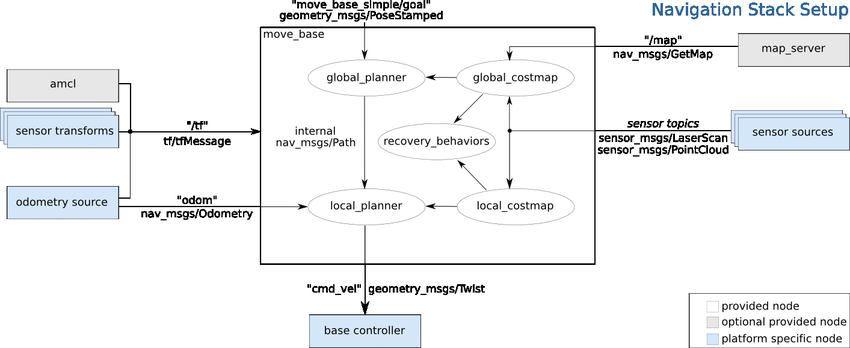
\includegraphics[width=0.8\textwidth]{Init/gambar/ros_nav.png}
    \caption[Diagram arsitektur ROS Navigation Stack]{Diagram arsitektur ROS Navigation Stack \cite{prague2016navstack}}
    \label{fig:ros_nav}
\end{figure}

Sebagaimana diilustrasikan pada Gambar \ref{fig:ros_nav}, fungsionalitas pergerakan otonom di dalam ekosistem ROS difasilitasi oleh kumpulan pustaka dan modul terintegrasi yang dikenal sebagai \textit{Navigation Stack}. Arsitektur navigasi ini berpusat pada \textit{move\_base}, sebuah \textit{node} koordinator yang mengintegrasikan aliran informasi dari berbagai sistem, termasuk \textit{transform tree} (TF) untuk melacak relasi spasial, data peta spasial, pembacaan sensor LiDAR, dan telemetri odometri robot. Ketika \textit{move\_base} menerima sebuah target koordinat tujuan (\textit{goal pose}) dalam bentuk pesan \textit{Action}, ia meneruskan data persepsi tersebut ke modul perencana jalur global (\textit{global planner}) dan lokal (\textit{local planner}) secara bertahap. Hasil akhir dari pemrosesan di dalam \textit{node} navigasi ini adalah pengiriman perintah gerak secara berkala melalui \textit{topic} yang mengatur kecepatan linier dan sudut (\textit{cmd\_vel}). Perintah ini selanjutnya diterjemahkan oleh unit pengendali perangkat keras (\textit{hardware controller}) menjadi putaran motor yang menggerakkan robot menuju tujuannya. Dalam penelitian ini, \textit{Navigation Stack} digunakan sebagai kerangka utama yang mengoordinasikan seluruh proses navigasi robot \textit{quadruped}, mulai dari penerimaan tujuan yang dikirimkan oleh agen LLM hingga eksekusi gerakan fisik di lingkungan pabrik.

\subsubsection{\textit{Rosbridge Suite}}
\textit{Rosbridge Suite} adalah lapisan \textit{middleware} yang dirancang untuk menjembatani komunikasi antara ekosistem ROS dengan aplikasi eksternal yang tidak berbasis ROS, seperti aplikasi antarmuka web atau klien jarak jauh \cite{crick2016rosbridge}. Komponen ini bekerja dengan menyediakan antarmuka \textit{Application Programming Interface} (API) berbasis JSON (\textit{JavaScript Object Notation}) yang dapat diakses melalui standar komunikasi \textit{WebSocket}. Melalui \textit{rosbridge}, aplikasi pihak ketiga dapat melakukan operasi fundamental ROS secara langsung di atas jaringan, seperti mempublikasikan (\textit{publish}) data ke suatu \textit{topic}, berlangganan (\textit{subscribe}) untuk menerima aliran data sensor, atau memanggil layanan (\textit{services}) tanpa perlu menginstal pustaka ROS secara penuh di sisi klien. Dalam arsitektur sistem robot inspeksi yang terhubung ke internet, \textit{rosbridge} memegang peranan esensial sebagai jalur komunikasi utama yang memfasilitasi pengiriman perintah dari \textit{dashboard} kontrol maupun \textit{Large Language Model}, sekaligus menyalurkan telemetri dan data pandangan robot secara \textit{real-time} kembali ke pengguna.


\subsection{Lokalisasi dan Pemetaan}
Lokalisasi dan pemetaan merupakan kemampuan fundamental yang saling bergantung bagi robot otonom untuk dapat beroperasi dan menavigasi lingkungan yang kompleks secara presisi. Dalam disiplin ilmu robotika, proses memetakan lingkungan sekaligus menentukan posisi robot di dalamnya diistilahkan sebagai \textit{Simultaneous Localization and Mapping} (SLAM). Menurut Thrun dkk. \cite{stachniss2016simultaneous}, SLAM adalah kerangka dasar bagi robot otonom sejati karena mengizinkan sistem untuk memahami lingkungan yang tidak terstruktur tanpa perlu bergantung pada instrumen penentuan posisi eksternal. Secara teknis, proses pemetaan bertugas membangun representasi tata letak rintangan di sekeliling robot berdasarkan data sensor, sementara proses lokalisasi secara terus-menerus menggunakan peta tersebut untuk mengestimasi letak dan arah robot. Gabungan dari kedua kemampuan pemetaan ruang ini menjadi fondasi penting dalam pengembangan proyek robot inspeksi \textit{quadruped}, yang mensyaratkan tersedianya peta 3D lingkungan sebelum sistem dapat menjalankan misi navigasi secara otonom berdasarkan instruksi dari \textit{Large Language Model}.

\subsubsection{\textit{Graph} SLAM}

\begin{figure}[H]
    \centering
    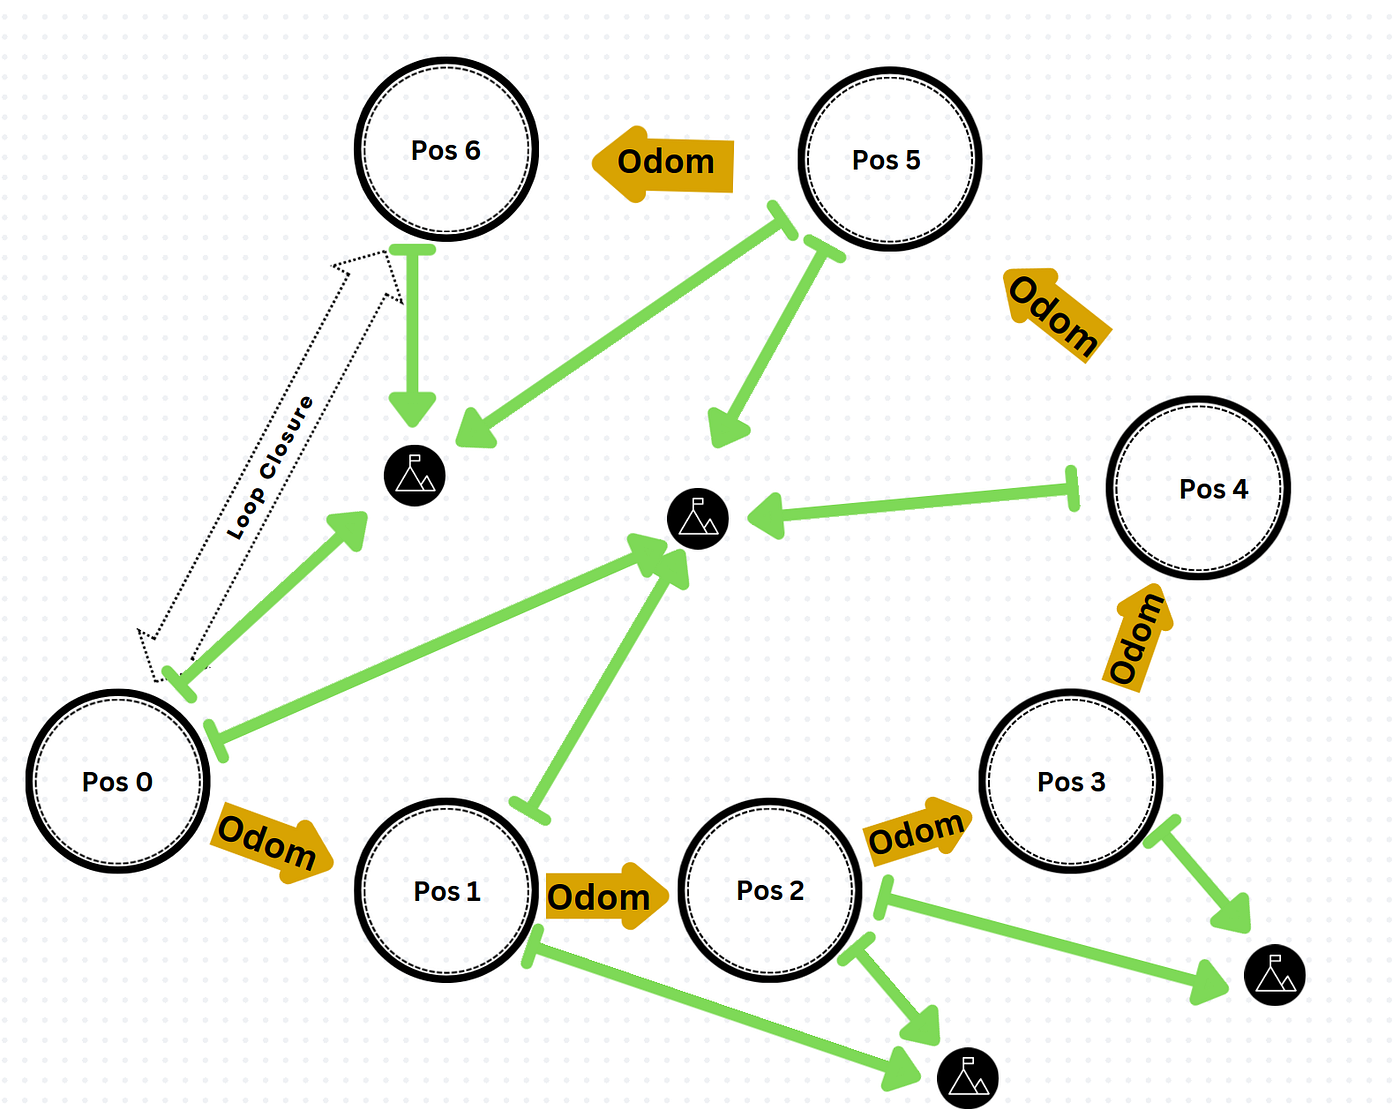
\includegraphics[width=0.65\textwidth]{Init/gambar/graph_slam.png}
    \caption[Diagram Graph SLAM]{Diagram Graph SLAM \cite{rustam2024graphslam}}
    \label{fig:graph_slam}
\end{figure}

Berdasarkan skema pada Gambar \ref{fig:graph_slam}, \textit{Graph SLAM} adalah pendekatan pemetaan yang merepresentasikan riwayat perjalanan robot sebagai sebuah graf posisi (\textit{pose graph}), di mana setiap simpul (\textit{node}) mewakili pose robot pada waktu tertentu dan setiap \textit{edge} mewakili kendala spasial yang diturunkan dari data sensor maupun odometri. Metode ini secara fundamental memformulasikan SLAM sebagai persoalan optimasi graf, di mana akumulasi kesalahan estimasi jarak (\textit{drift}) dapat dikoreksi secara menyeluruh melalui mekanisme pengenalan area berulang (\textit{loop closure}) yang memperbarui seluruh riwayat rute secara konsisten. Dalam konteks implementasi pada sistem berbasis LiDAR, Koide dkk. \cite{koide2019portable} mengembangkan \textit{hdl\_graph\_slam}, sebuah implementasi Graph SLAM yang portabel dan efisien untuk pemetaan 3D menggunakan sensor LiDAR. Implementasi ini memanfaatkan kombinasi algoritma \textit{scan matching} dan optimasi graf untuk menghasilkan peta 3D berkualitas tinggi secara \textit{real-time}. Penggunaan kerangka kerja ini dalam penelitian memastikan bahwa robot \textit{quadruped} dapat menghasilkan peta 3D lingkungan pabrik yang presisi sebagai panduan utama untuk proses penentuan lokasi dan navigasi otonom.

% \subsubsection{Normal Distributions Transform (NDT)}
% \textit{Normal Distributions Transform} (NDT) merupakan algoritma pencocokan pemindaian (\textit{scan matching}) yang efisien karena menyelaraskan dua himpunan \textit{point cloud} dengan memodelkannya ke dalam probabilitas distribusi spasial. Biber dan Stra{\ss}er \cite{biber2003normal} mengemukakan rumusan NDT yang bekerja dengan membagi ruang ke dalam sel-sel berukuran tetap dan merepresentasikan titik-titik permukaan di dalam setiap sel menggunakan matriks kovariansi dan nilai rata-rata dari distribusi Gaussian. Melalui implementasi paralelisasi komputasi (\textit{multi-threading}), pemetaan probabilitas ini menghilangkan kebutuhan komputasi berat untuk mencari korespondensi individual dari titik-ke-titik secara persis saat meregistrasikan sensor LiDAR baru ke \textit{global map} 3D. Kemampuan matematis NDT yang efisien memberikan kepastian perhitungan \textit{pose} (posisi dan orientasi) secara \textit{real-time}, sehingga robot selalu dapat mengeksekusi manuver navigasi spasialnya tanpa lag komputasi yang berbahaya.

\subsubsection{\textit{Fast-Generalized Iterative Closest Point} (Fast-GICP)}
\textit{Fast-Generalized Iterative Closest Point} (Fast-GICP) adalah algoritma optimasi dari GICP standar yang difokuskan untuk mengakselerasi tahap kalkulasi matriks transformasi pada registrasi \textit{point cloud} 3D. Koide dkk. \cite{koide2021voxelized} mengembangkan varian efisien \textit{Fast-GICP} yang menerapkan paralelisasi dan struktur data berbasis \textit{voxel} sehingga mampu mempertahankan keakuratan yang ekuivalen dengan GICP standar sembari menekan latensi komputasi secara masif. Di dalam lapisan persepsi robot, algoritma ini menangani data \textit{point cloud} berskala besar dengan lebih ringkas karena struktur voksel secara dramatis meminimalkan redundansi pencarian titik terdekat (\textit{nearest-neighbor matching}) yang secara konvensional menjadi \textit{bottleneck} komputasi. Pemanfaatan kapabilitas pencocokan super cepat dari \textit{Fast-GICP} ini berdampak langsung pada modul perencanaan (\textit{planning}), yang memampukan robot \textit{quadruped} untuk mengenali letak dirinya secara instan dan bereaksi lincah terhadap rintangan di area pabrik industri.

\subsection{Navigasi}
Sistem navigasi otonom adalah kapabilitas pengambilan keputusan yang memungkinkan robot untuk menentukan dan mengeksekusi lintasan pergerakan paling aman dari titik awal menuju lokasi target. Pada arsitektur operasional robot tingkat lanjut, proses navigasi dikendalikan melalui pengontrol terpusat yang bersifat hierarkis \cite{quigley2009ros}. Sistem ini beroperasi dengan memecah permasalahan lintasan menjadi dua lapisan independen: \textit{Global Planner} untuk menentukan jalur keseluruhan secara makro, dan \textit{Local Planner} untuk menerjemahkan jalur tersebut menjadi perintah kendali motor reaktif. Pembagian kerja ini memisahkan perhitungan rute jarak jauh yang hanya membutuhkan analisis peta statis, dari kebutuhan kalkulasi menghindar rintangan (\textit{obstacle avoidance}) secara refleksif yang sangat sensitif terhadap latensi waktu. Koordinasi antara kedua tingkat perencanaan ini sangat dibutuhkan agar robot \textit{quadruped} dapat melaksanakan inspeksi ke berbagai titik komponen secara efisien dan aman.

\subsubsection{Algoritma \textit{Shortest Path} Dijkstra sebagai \textit{Global Planner}}
\textit{Global Planner} adalah perencana jalur tingkat makro yang bertugas mengkalkulasi lintasan rute terpendek secara absolut di atas referensi peta statis (\textit{global map}). Untuk melakukan kalkulasi rute, lapisan ini seringkali memanfaatkan algoritma \textit{shortest path} seperti Dijkstra \cite{dijkstra2022note}, yaitu metode matematis yang menjamin penemuan rute terpendek dari satu titik awal ke semua titik lain pada peta. Algoritma ini membaca \textit{grid cells} dari peta, lalu menghitung jarak kumulatif dari setiap area yang belum dikunjungi hingga menemukan titik akhir tujuan. Penggunaan Dijkstra dinilai ideal dibandingkan algoritma alternatif seperti \textit{A-Star} (A*) apabila tujuannya adalah mendapatkan jaminan jalur yang paling mulus (\textit{smooth}) dan stabil dari berbagai arah, meskipun membutuhkan proses perhitungan awal yang sedikit lebih berat. Jaminan rute terpendek yang dihasilkan algoritma ini memastikan bahwa robot dapat bergerak seefisien mungkin tanpa membuang daya baterai.

Secara matematis, pembaruan jarak minimum pada algoritma Dijkstra untuk setiap simpul $v$ yang berdekatan dengan simpul $u$ diformulasikan sebagai berikut:

\begin{equation}
d(v) = \min(d(v), d(u) + w(u, v))
\label{eq:dijkstra}
\end{equation}

di mana $d(v)$ adalah jarak terpendek sementara dari titik awal ke simpul $v$, $d(u)$ adalah jarak terpendek yang telah diketahui ke simpul $u$, dan $w(u, v)$ adalah bobot atau jarak lintasan dari simpul $u$ ke simpul $v$.

\subsubsection{\textit{Timed Elastic Band} sebagai \textit{Local Planner}}
\textit{Timed Elastic Band} (TEB) adalah algoritma \textit{Local Planner} tingkat mikro yang secara dinamis memodifikasi trayektori jalur global untuk menghindari tabrakan secara \textit{real-time}. Diperkenalkan oleh R{\"o}smann dkk. \cite{rosmann2012trajectory}, pendekatan TEB bekerja dengan cara mengoptimalkan jalur secara terus-menerus menyerupai karet elastis yang dapat ditarik atau didorong menjauhi rintangan, sembari sangat mempertimbangkan batasan kinematik dan dinamik dari robot otonom. Secara konseptual, TEB diatur agar mampu menyesuaikan diri dengan cara berjalan fisik dari robot, baik itu gaya gerak segala arah (\textit{holonomik}) maupun terbatas (\textit{non-holonomik}). Algoritma ini secara langsung memperhitungkan batas kemampuan perangkat seperti batas percepatan maksimum, batas kecepatan maju, hingga batas radius putaran. Dengan perhitungan ini, pergerakan robot saat menghindari objek bergerak akan selalu terlihat halus dan tetap seimbang. Penerapan sistem lapis pelindung TEB ini memastikan bahwa ketika program AI mengirimkan urutan tujuan yang sulit, robot tetap bisa bereaksi dengan gesit dan berbelok dengan aman, sekalipun berada di area kerja yang ramai dengan aktivitas.

Secara matematis, TEB memformulasikan masalah perencanaan lintasan lokal sebagai persoalan optimasi multi-objektif. Fungsi objektif yang diminimalkan merupakan kombinasi berbobot dari berbagai fungsi \textit{cost} kendala kinematik dan spasial:

\begin{equation}
f(\mathbf{B}) = \sum_{k} \gamma_k f_k(\mathbf{B})
\label{eq:teb_objective}
\end{equation}

di mana $\mathbf{B}$ merepresentasikan urutan konfigurasi pose robot dan interval waktu antar pose, $f_k(\mathbf{B})$ adalah fungsi-fungsi \textit{cost} spesifik (seperti optimasi waktu tempuh, jarak dari rintangan, dan pemenuhan batasan kecepatan), serta $\gamma_k$ adalah parameter bobot untuk masing-masing fungsi \textit{cost} tersebut.

\subsection{\textit{Model Context Protocol} (MCP)}

\begin{figure}[H]
    \centering
    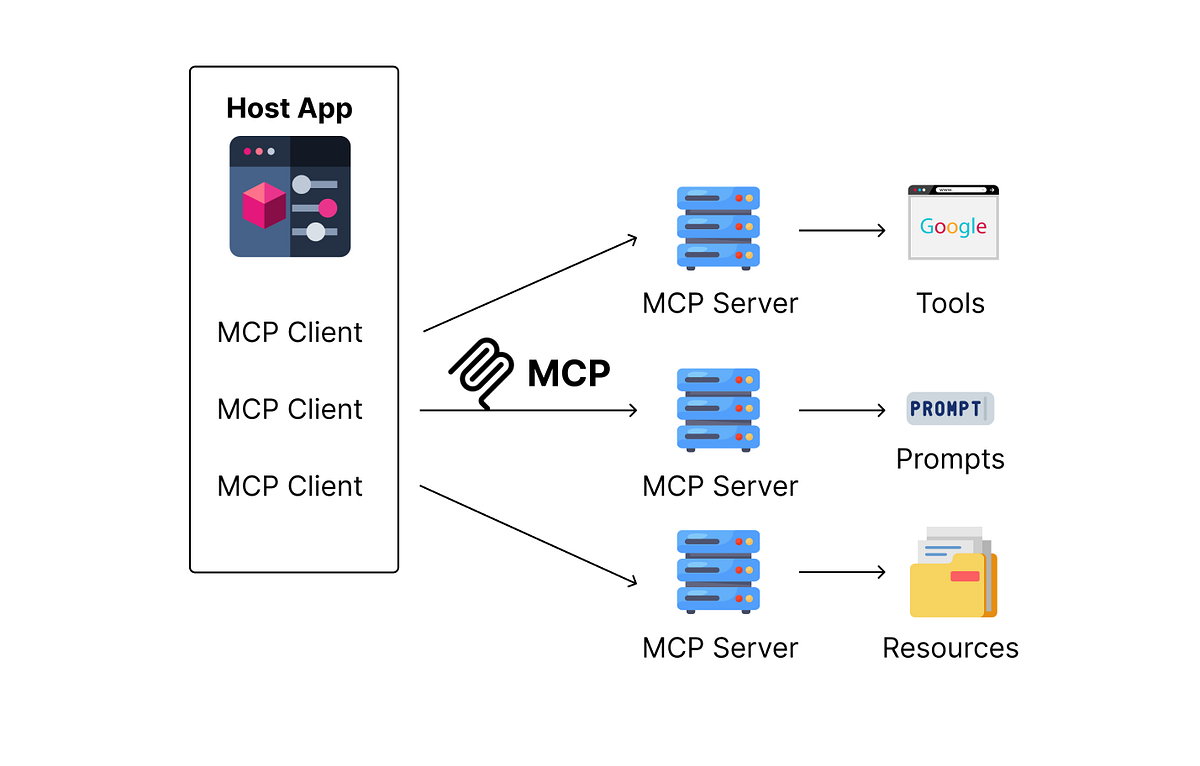
\includegraphics[width=0.8\textwidth]{Init/gambar/mcp.png}
    \caption[Diagram arsitektur MCP]{Diagram arsitektur MCP \cite{zhao2025mcp}}
    \label{fig:mcp}
\end{figure}

Seperti yang ditunjukkan oleh arsitektur pada Gambar \ref{fig:mcp}, \textit{Model Context Protocol} (MCP) adalah sebuah antarmuka terstandarisasi yang dirancang untuk memungkinkan interaksi yang lancar antara model AI dengan \textit{tools} dan sumber daya eksternal. Tujuan utama protokol ini adalah mengatasi masalah isolasi data dan memfasilitasi interoperabilitas di antara berbagai sistem yang berbeda. Sebelum adanya MCP, pengembang harus membuat koneksi API secara manual untuk setiap layanan eksternal (n-to-n connection). Sebaliknya, MCP menyediakan sebuah lapisan abstraksi universal, di mana aplikasi AI (sebagai MCP Client) dapat berkomunikasi dengan berbagai \textit{tools} melalui perantara yang disebut MCP Server, mengubah pola koneksi menjadi 1-to-n yang lebih efisien \cite{hou2025model}.

\subsubsection{Komponen MCP} Berdasarkan tinjauan oleh Hou et al. \cite{hou2025model}, arsitektur MCP dibangun di atas tiga komponen fundamental yang saling berinteraksi secara sinergis. Komponen pertama adalah MCP Host, yang merupakan aplikasi utama tempat model AI dijalankan, seperti \textit{Integrated Development Environment} (IDE) atau aplikasi antarmuka obrolan. Host ini bertindak sebagai wadah (\textit{container}) bagi proses AI. Di dalam ekosistem tersebut, terdapat MCP Client yang berfungsi sebagai jembatan komunikasi di dalam Host. Client bertanggung jawab penuh untuk mengelola koneksi 1:1 dengan Server, mengirimkan permintaan pengguna, dan menangani respons balik. Dalam penelitian ini, peran tersebut dijalankan oleh skrip Python yang mengelola sesi obrolan. Komponen terakhir adalah MCP Server, yang bertugas mengekspos kemampuan teknis kepada AI. Server ini menyediakan tiga jenis primitif utama, yaitu \textit{Tools} yang merupakan fungsi eksekusi seperti navigasi robot atau API query, \textit{Resources} yang berisi data yang dapat dibaca seperti file log atau database, serta \textit{Prompts} yang menyediakan templat instruksi yang telah ditentukan sebelumnya. Dengan arsitektur ini, MCP memungkinkan model AI untuk secara dinamis menemukan dan memilih alat yang dibutuhkan sesuai dengan konteks tugas yang sedang dihadapi \cite{singh2025survey}.

\subsubsection{Protokol Transportasi MCP} Komunikasi antara Client dan Server dalam ekosistem MCP difasilitasi oleh dua mekanisme transportasi standar yang dipilih berdasarkan arsitektur jaringan sistem. Metode pertama adalah Standard Input/Output (stdio), yang digunakan khusus untuk komunikasi lokal di mana Client meluncurkan Server sebagai sub-proses. Metode ini menawarkan keunggulan berupa latensi yang sangat rendah dan tingkat keamanan yang tinggi karena proses tidak terekspos ke jaringan luar. Sebagai alternatif untuk komunikasi jarak jauh dan terdistribusi, digunakan mekanisme HTTP dengan Server-Sent Events (SSE). Dalam mode ini, Server berjalan sebagai layanan web independen, di mana Client mengirimkan perintah melalui HTTP POST dan menerima pembaruan atau notifikasi kejadian (events) secara \textit{real-time} melalui SSE. Metode kedua inilah yang diterapkan dalam penelitian ini untuk menghubungkan antarmuka obrolan dengan server robot yang berjalan di lingkungan terisolasi (Docker).

\subsection{\textit{Large Language Models} (LLM)}
\textit{Large Language Models} (LLM) merupakan model komputasi canggih yang dibangun di atas arsitektur jaringan saraf tiruan, khususnya arsitektur \textit{Transformer}, yang dilatih menggunakan korpus data teks dalam skala masif. Kemampuan fundamental LLM terletak pada proses prediksi \textit{token} atau kata berikutnya dalam sebuah urutan (\textit{next-token prediction}). Proses ini memungkinkan model untuk memelajari tata bahasa, konteks, penalaran, dan pengetahuan umum dari data latihnya secara mendalam. Arsitektur \textit{Transformer}, dengan mekanisme \textit{self-attention}, sangat efektif dalam menangani dependensi jarak jauh (\textit{long-range dependencies}) dalam teks, sehingga model dapat memahami konteks dari sebuah kalimat atau paragraf secara utuh dan komprehensif \cite{chang2024survey}. Dalam penelitian ini, LLM berperan sebagai otak utama agen robot yang menerjemahkan instruksi bahasa alami dari operator menjadi rangkaian perintah navigasi dan inspeksi yang dapat dieksekusi secara langsung oleh sistem robotik.

\subsubsection{\textit{Agentic} AI}
Perkembangan terbaru dalam bidang kecerdasan buatan telah mendorong evolusi \textit{Large Language Models} (LLM) dari sekadar mesin pemroses teks pasif menjadi \textit{autonomous agents} yang mampu berinteraksi secara aktif dengan lingkungannya demi mencapai tujuan tertentu. Xi et al. \cite{xi2025rise} mendefinisikan agen berbasis LLM sebagai sistem yang memanfaatkan model bahasa besar sebagai pengendali utama atau otak untuk mempersepsikan lingkungan, mengambil keputusan, dan mengeksekusi tindakan. Berbeda dengan LLM standar yang kemampuannya terbatas pada menghasilkan teks atau saran konseptual, Agentic AI memanfaatkan pemahaman semantiknya sebagai landasan untuk merumuskan dan mengeksekusi tindakan nyata. Kemampuan inilah yang memungkinkan sistem untuk tidak sekadar merespons instruksi abstrak secara pasif, melainkan beradaptasi dengan skenario yang tidak terduga melalui interaksi otonom menggunakan alat bantu (\textit{tools}) eksternal.

Secara arsitektural, Wang et al. \cite{wang2024survey} merumuskan kerangka kerja \textit{agent} ke dalam empat komponen fundamental yang saling terintegrasi, yaitu profil agen, memori, perencanaan, dan tindakan. Komponen perencanaan (\textit{planning}) memainkan peran krusial dalam sistem robotik, di mana \textit{agent} harus memecah instruksi tingkat tinggi yang kompleks menjadi serangkaian sub-tugas yang dapat dieksekusi atau \textit{Chain of Thought}. Kemampuan ini memungkinkan \textit{agent} untuk melakukan dekomposisi masalah dan refleksi diri, sehingga dapat memperbaiki rencana jika menemui kegagalan saat eksekusi. Sementara itu, komponen memori memungkinkan \textit{agent} untuk menyimpan riwayat interaksi dan pengetahuan prosedural, menciptakan pengalaman pengguna yang kontinu dan kontekstual. Dalam penelitian ini, arsitektur \textit{agentic} diimplementasikan melalui \textit{agent} LLM yang memiliki akses langsung ke \textit{tools} navigasi dan inspeksi robot melalui MCP Server.

\subsubsection{Penggunaan \textit{Tools} dan \textit{Model Context Protocol} (MCP)}
Salah satu kapabilitas LLM modern yang paling signifikan adalah kemampuan \textit{tool use} atau penggunaan alat. Dalam ekosistem pengembangan \textit{agent}, \textit{tools} dalam konteks \textit{Model Context Protocol} (MCP) didefinisikan sebagai kapabilitas eksekusi yang diekspos oleh server, yang memberdayakan LLM untuk melakukan aksi nyata, berinteraksi dengan sistem eksternal, dan menjalankan operasi dinamis di luar sekadar memberikan respons teks statis \cite{singh2025survey}.

Berbeda dengan sumber data pasif, \textit{tools} dirancang untuk pemanggilan aktif oleh model. Mekanisme ini secara signifikan memperluas fungsionalitas \textit{agentic} dari sistem berbasis LLM. Ketika LLM mendeteksi bahwa permintaan pengguna memerlukan interaksi sistem (seperti mengambil data sensor atau menggerakkan robot), model akan menghasilkan \textit{output} terstruktur yang sesuai dengan skema JSON yang telah didefinisikan. Skema ini merinci parameter input dan validasi untuk memastikan eksekusi perintah yang aman dan presisi pada sistem target \cite{singh2025survey}.

\subsubsection{\textit{Multimodal Large Language Models} (MLLM)}
Sejalan dengan kebutuhan interaksi yang lebih kompleks, LLM telah berevolusi menjadi \textit{Multimodal Large Language Models} (MLLM). Ekstensi arsitektural ini memampukan model bahasa untuk tidak hanya memproses dan memahami teks, tetapi juga menerima berbagai jenis modalitas data lain seperti \textit{image}, video, dan audio sebagai masukannya \cite{yin2024survey}. Proses perpaduan ragam data ini diwujudkan melalui komponen enkoder khusus (seperti \textit{vision encoder}) yang bertugas mengekstraksi fitur visual, lalu menggunakan mekanisme penyelarasan (\textit{alignment}) untuk memetakan representasi fitur tersebut ke dalam ruang laten bahasa yang sama. Dalam ranah robotika, kehadiran MLLM menawarkan lompatan kapabilitas persepsi yang besar. Alih-alih bergantung pada sistem penglihatan komputer (\textit{computer vision}) tradisional yang sempit kemampuannya, robot kini dapat memahami dan menalar apa yang dilihat oleh kameranya yang kemudian dijelaskan kembali secara kontekstual menggunakan bahasa alami. Hal ini memungkinkan robot inspeksi untuk memproses konteks visual lingkungannya secara utuh guna melakukan analisis mendalam terhadap objek-objek inspeksi.


\subsection{Interaksi Manusia-Robot (\textit{Human-Robot Interaction})}
\textit{Human-Robot Interaction} (HRI) merupakan bidang studi multidisiplin yang berfokus pada perancangan, evaluasi, dan pemahaman mekanisme interaksi antara manusia dan robot dengan tujuan utama menciptakan kolaborasi yang aman, efisien, dan alami. Dalam spektrum metode interaksi yang ada, penggunaan bahasa alami (\textit{natural language}) dianggap sebagai salah satu pendekatan paling menjanjikan karena meminimalisasi hambatan komunikasi, memungkinkan pengguna untuk berinteraksi dengan robot tanpa memerlukan pelatihan teknis khusus atau pemahaman antarmuka grafis yang rumit \cite{mavridis2015review}. Dengan memampukan robot untuk memproses instruksi tingkat tinggi dalam bahasa sehari-hari seperti perintah "periksa area di sebelah kanan", sistem HRI berbasis bahasa alami dapat secara signifikan menurunkan beban kognitif operator. Hal ini memungkinkan perhatian operator dialihkan dari mekanisme kontrol ke tujuan strategis misi.

Efektivitas sebuah sistem HRI tidak hanya diukur dari kemampuan robot dalam menerjemahkan perintah input, tetapi juga dari kapasitasnya dalam memberikan umpan balik yang komprehensif kepada operator. Kemampuan robot untuk melaporkan status operasional, intensi pergerakan, atau temuan inspeksi secara verbal maupun sangat krusial dalam membangun pemahaman situasi. Dalam konteks tugas inspeksi industri, transparansi informasi ini memastikan operator memahami apa yang sedang dipersepsikan oleh robot secara \textit{real-time}. Hal ini mengubah peran operator dari sekadar pengendali alat menjadi supervisor misi, di mana kompleksitas penerjemahan sinyal teknis dan pelaporan status ditangani secara otonom oleh sistem cerdas, yang pada akhirnya mempercepat adopsi teknologi robotik di lingkungan kerja yang kompleks.

Integrasi \textit{Large Language Models} (LLM) ke dalam arsitektur HRI memperkuat hal ini dengan menawarkan fleksibilitas yang tidak dimiliki oleh sistem berbasis \textit{hard-coded}. Berbeda dengan sistem tradisional yang memerlukan perintah spesifik, HRI yang ditenagai oleh LLM mampu menangani ambiguitas bahasa dan menyimpulkan konteks implisit dari instruksi operator. Kemampuan ini sangat relevan untuk robot inspeksi otonom, di mana instruksi sering kali bersifat dinamis dan bergantung pada situasi lingkungan yang tidak terduga.

\subsubsection{Mekanisme \textit{Human-in-the-Loop} (HITL)}
\textit{Human-in-the-Loop} (HITL) adalah sebuah pendekatan dalam sistem otonom dan kecerdasan buatan yang secara eksplisit mengintegrasikan intervensi manusia ke dalam siklus operasional sistem. Dalam konteks robotika otonom, konsep ini menempatkan operator manusia tidak hanya sebagai pengamat pasif, melainkan sebagai supervisor aktif yang memiliki otoritas untuk memverifikasi, memodifikasi, atau membatalkan keputusan yang diambil oleh agen AI sebelum dan saat instruksi dieksekusi. Penerapan HITL menjadi sangat krusial pada sistem berbasis \textit{Agentic AI} dan \textit{Large Language Models} untuk memitigasi risiko kegagalan sistem akibat halusinasi atau kesalahan penalaran yang melekat pada model parametrik. Melalui mekanisme ini, batas antara otonomi penuh dan kontrol manual dijembatani, sehingga sistem tetap dapat memanfaatkan kecepatan komputasi AI dalam merencanakan rute atau menganalisis lingkungan, sekaligus memastikan keandalan operasional melalui penilaian operator saat menghadapi kondisi lingkungan industri yang dinamis dan tidak terduga.

\subsection{\textit{Retrieval-Augmented Generation} (RAG)}
\textit{Retrieval-Augmented Generation} (RAG) adalah sebuah teknik dalam pemrosesan bahasa alami yang menggabungkan kekuatan model bahasa parametrik dengan memori non-para-metrik yang berasal dari indeks vektor eksternal. Konsep ini pertama kali diperkenalkan secara formal oleh Lewis et al. \cite{lewis2020retrieval} untuk mengatasi keterbatasan pada \textit{Large Language Models} (LLM), yaitu ketidakmampuan untuk mengakses informasi terkini setelah proses pelatihan selesai serta kecenderungan untuk menghasilkan halusinasi atau informasi yang tidak akurat ketika dihadapkan pada topik spesifik yang jarang muncul dalam data latih.

Dalam arsitektur RAG standar, proses inferensi dibagi menjadi dua fase utama, yaitu fase pencarian (\textit{retrieval}) dan fase pembangkitan (\textit{generation}). Ketika model menerima masukan dari pengguna, sistem terlebih dahulu melakukan pencarian semantik menggunakan indeks vektor padat untuk mengambil dokumen yang relevan dari pengetahuan eksternal. Dokumen-dokumen ini kemudian digabungkan dengan pertanyaan asli sebagai konteks tambahan yang diberikan kepada generator untuk menghasilkan respons. Pendekatan ini memungkinkan model untuk memberikan jawaban yang lebih faktual, spesifik, dan dapat diverifikasi sumbernya, yang sangat krusial untuk aplikasi inspeksi di mana akurasi data SOP adalah prioritas utama.

\subsubsection{\textit{Agentic} RAG}
Seiring berkembangnya kompleksitas tugas yang harus diselesaikan oleh AI, RAG telah berevolusi dari sekadar pengambilan informasi pasif menjadi sistem yang lebih otonom yang dikenal sebagai Agentic RAG. Perbedaan mendasar antara RAG standar dan Agentic RAG terletak pada mekanisme kontrol dan kemampuan penalaran. Pada RAG standar, alur kerja bersifat linier dan deterministik yang dimulai dari proses pencarian informasi, dilanjutkan dengan pembacaan konteks, dan diakhiri dengan pembuatan respons. Sistem akan selalu mengambil dokumen setiap kali ada pertanyaan tanpa mengevaluasi urgensi atau relevansi dokumen tersebut terhadap konteks permasalahan \cite{gao2023retrieval}.

Sebaliknya, Agentic RAG mengintegrasikan kemampuan \textit{Reasoning and Acting} (ReAct) sebagaimana diusulkan oleh Yao et al. \cite{yao2022react}. Dalam kerangka kerja ini, LLM bertindak sebagai agen otonom yang memiliki serangkaian kemampuan kognitif tingkat lanjut. Agen mampu melakukan perencanaan mandiri untuk memecah pertanyaan kompleks menjadi sub-tugas yang lebih kecil, serta memiliki kemampuan penggunaan alat (\textit{tool use}) untuk memilih secara dinamis kapan harus menggunakan mesin pencari dan kapan cukup menggunakan pengetahuan internalnya. Selain itu, agen juga menerapkan evaluasi multi-langkah di mana hasil pencarian diverifikasi terlebih dahulu. Jika informasi dirasa kurang memadai, agen dapat memutuskan untuk melakukan pencarian ulang guna menciptakan siklus umpan balik sebelum memberikan jawaban akhir. Pendekatan agentic ini memungkinkan implementasi sistem inspeksi yang fleksibel, di mana robot tidak hanya menjawab pertanyaan berdasarkan dokumen, tetapi dapat menavigasi dan mengambil keputusan operasional secara bertahap berdasarkan informasi yang diperoleh secara \textit{real-time}.


%\end{landscape}
\subsection{Supabase}
\textit{Supabase} adalah platform layanan basis data \textit{open-source} yang dibangun di atas sistem manajemen basis data relasional PostgreSQL. Layanan \textit{Backend-as-a-Service} (BaaS) ini menggabungkan keandalan basis data terstruktur dengan kemudahan akses API modern. Secara teknis, Supabase bekerja dengan cara secara otomatis membangkitkan REST API dari skema tabel yang dibuat oleh pengembang, sehingga operasi \textit{read} dan \textit{write} data dapat langsung dilakukan melalui permintaan HTTP tanpa perlu menulis logika server tambahan. Selain itu, platform ini mendukung langganan data waktu-nyata (\textit{realtime subscriptions}) melalui protokol \textit{WebSocket}, yang memungkinkan antarmuka klien menerima pembaruan data secara instan. Sistem Supabase berperan krusial sebagai repositori histori percakapan antara operator dan sistem robot, dan basis pengetahuan memori untuk sistem RAG (\textit{Retrieval-Augmented Generation}). Seluruh rekaman data historis ini dapat ditarik (\textit{query}) oleh modul LLM server secara cepat untuk menjaga keberlanjutan konteks percakapan di setiap sesi operasi robot.



